\documentclass[12pt, addpoints]{exam/exam}

\usepackage{hyperref}
%\usepackage{mdframed}
\usepackage{graphicx, caption}	
%\usepackage{array, multicol, tabu}
\usepackage{amsmath, amsthm, amssymb}
\usepackage{comment}
\usepackage{enumitem}
\usepackage{url}
\usepackage{textcomp}
\usepackage{wrapfig}
\usepackage{multicol}

\newcommand{\1}{^{-1}}
\newcommand{\vect}[1]{\mathbf{#1}}
\newcommand{\R}{\mathbb R}
\newcommand{\vstr}{\vspace{\stretch{1}}}
\everymath{\displaystyle}
\setlength{\parindent}{0pt}

\theoremstyle{plain}
\newtheorem{thm}{Theorem}
\newtheorem*{thm*}{Theorem}

%\printanswers
\pointformat{\bf(\thepoints)}
\pointpoints{pt}{pts}
\bonuspointformat{\bf(\thepoints)}
\bonuspointpoints{pt}{pts}

\coverfirstpageheader{\bf MATH 235 (Calculus I) \\
		Fall 2017 \\
		}
		{}
		{{Name:} \underline{\hspace{40ex}} \\
		\vspace{0.5pc}
		Mon 11 Dec 2017}
\coverextraheadheight[2pc]{0in}
\coverfirstpagefooter{}{}{\Large Good luck!}
\coverrunningheader{}
	{Final Exam}
	{}
\coverrunningheadrule	
\coverrunningfootrule
\coverrunningfooter{Calc I Fall 2017}{}{p. \thepage\ (of \numpages)}

\firstpageheader{}
	{Final Exam}
	{}
\firstpageheadrule
\firstpagefootrule
\firstpagefooter{Calc I Fall 2017}{}{p. \thepage\ (of \numpages)}

\runningheadrule
\runningheader{}
	{Final Exam}
	{}
\runningfootrule
\runningfooter{Calc I Fall 2017}{}{p. \thepage\ (of \numpages)}

\title{\vspace{-8pc}
\vfill{\Huge
	\bf Final Exam %\\ 
	%(\S3.10, 4.1-4.6)
	} 
	}
%\author{}
\date{}

% % % % % % % % % % % % % % % % % % % %
\begin{document}

\begin{coverpages}
\maketitle
\thispagestyle{headandfoot}
\vspace{-4pc}
{\bf Exam Instructions:} You have 120 minutes to complete this exam.  \textbf{Justification} is required for all problems.  \textbf{Notation} matters!  You will also be penalized for \textbf{missing/incorrect units} and \textbf{rounding errors}. 

\vspace{1pc} 
No electronic devices (phones, iDevices, computers, etc) except for a basic scientific calculator.  On story problems, round to one decimal place.  If you do not have a calculator, then write down the exact formula you would plug in to a calculator to get the answer. 

\vspace{1pc}
If you finish early then you may leave, UNLESS there are less than 10 minutes left.  To prevent disruption, if you finish with less than 10 minutes remaining then please stay seated and quiet.

\begin{flushright}
%In addition, please provide the following data:

\vspace{0.3in}
%Drill Instructor: \underline{\hspace{40ex}}

\vspace{0.3in}
%Drill Time: \underline{\hspace{40ex}}
\end{flushright}

\vfill
\textbf{Your signature below indicates that you have read this page and agree to follow the Academic Honesty Policies of James Madison University.}  

\vspace{0.3in}
Signature: {\bf (1 pt)} \underline{\hspace{73ex}}

% % % % % % % % % %
\newpage
\vspace*{\fill}
\gradetable
%\textbf{Formulas you may need:}
%\vspace{-2pc}
%\begin{center}
%\vspace*{\fill}
%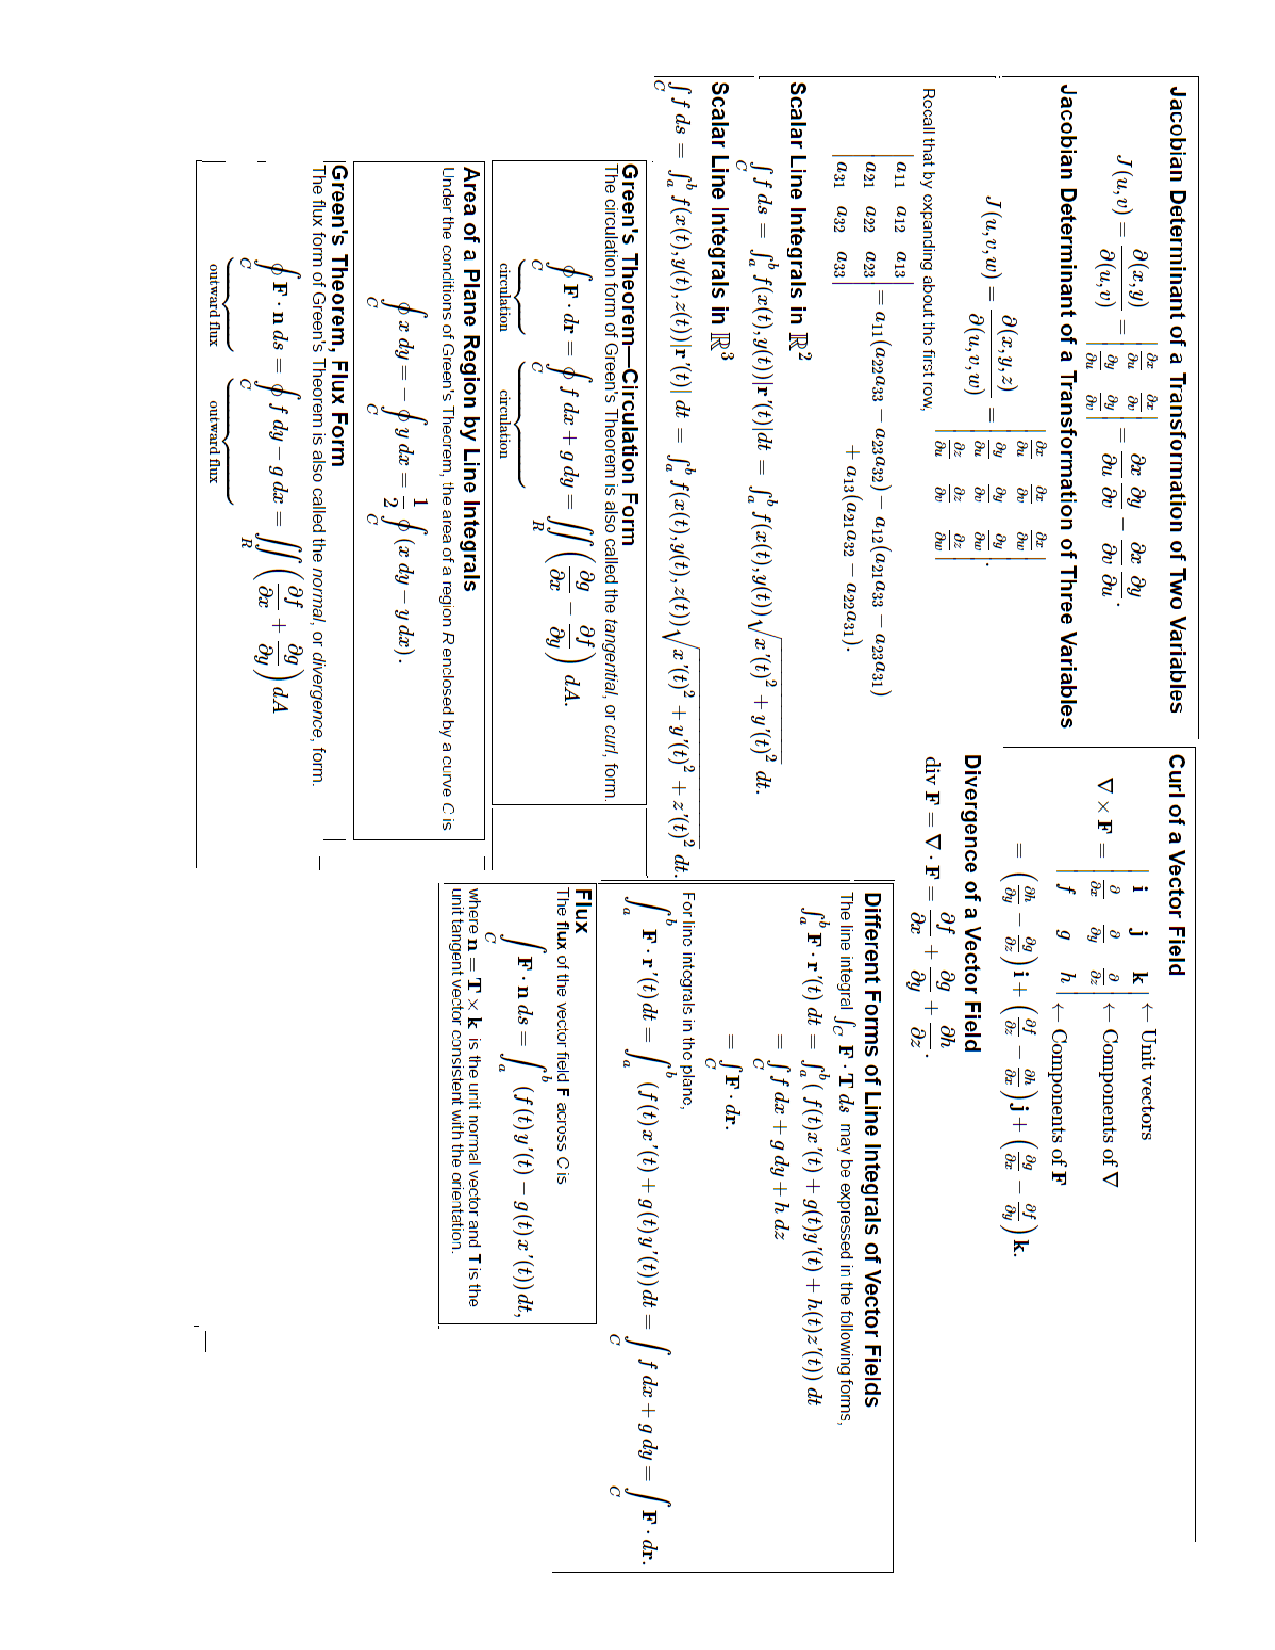
\includegraphics[scale=0.84]{Exam3FormulaSheet.pdf}
%\vspace*{\fill}
%\end{center}
\end{coverpages}

% % % % % % % % % % % % % % % % % % % %
\begin{questions}
\thispagestyle{headandfoot}

% % % % %
\question Determine whether each statement is TRUE or FALSE.  You will not receive full credit without justification of your answer. 
	\begin{parts}
	\part[2]%{\bf Ch 1 \#2} 
	If $f(s)=f(t)$, then $s=t$.
	\vspace{2.5pc}
	
	\part[2]%{\bf Ch 1 \#10} 
	If $x>0$, then $(\ln x)^6=6\ln x$.
	\vspace{2.5pc}
	
	\part[2]%{\bf Ch 1 \#14} 
	If $x$ is any real number, then $\sqrt{x^2}=x$.
	\vspace{2.5pc}
	
	\part[2]%{\bf Ch 2 \#12} 
	If $\lim_{x\to 0}f(x)=\infty$ and $\lim_{x\to 0}g(x)=\infty$, then $\lim_{x\to 0}\left(f(x)-g(x)\right)=0$.
	\vspace{2.5pc}
	
	\part[2]%{\bf Ch 2 \#18} 
	If $f$ is continuous on $[-1,1]$ and $f(-1)=4$ and $f(1)=3$, then there exists a number $c$ such that $|c|<1$ and $f(c)=\pi$.
	\vspace{2.5pc}
	
	\part[2]%{\bf Ch 3 \#2} 
	If $f$ and $g$ are differentiable, then $\frac{d}{dx}\left(f(x)g(x)\right)=f'(x)g'(x)$.
	\vspace{2.5pc}
	
	\part[2]%{\bf Ch 3 \#4} 
	If $f$ is differentiable, then $\frac{d}{dx}\sqrt{f(x)}=\frac{f'(x)}{2\sqrt{f(x)}}$.
	\vspace{2.5pc}
	
	\part[2]%{\bf Ch 3 \#8} 
	$\frac{d}{dx}(\ln{10})=\frac{1}{10}$
	\vspace{2.5pc}
	%\part {\bf Ch 3 \#14} An equation of the tangent line to the parabola $y=x^2$ at $(-2,4)$ is $y-4=2x(x+2)$.
	
	%\part[3]%{\bf Ch 5 \#2} 
	%If $f$ and $g$ are continuous on $[a,b]$, then
	%\[
	%\int_a^bf(x)g(x)\ dx = \left(\int_a^bf(x)\ dx\right)\left(\int_a^bg(x)\ dx\right).
	%\]
	%\vspace{1pc}
	
	\part[2]%{\bf Ch 5 \#6} 
	If $f'$ is continuous on $[1,3]$, then $\int_1^3f'(v)\ dv=f(3)-f(1)$. 
	\vspace{2.5pc}
	
	\part[2]%{\bf Ch 5 \#14} 
	If $\int_0^1f(x)\ dx=0$, then $f(x)=0$ for all $0\leq x\leq 1$.
	\vspace{2.5pc}
	\end{parts}

\newpage
% % % 
\question%{\bf Ch 1 \#6} 
Consider the function $g(x)=\sqrt{16-x^4}$.    
	\begin{parts}
	\part[2] Find the domain of $g$.
	\vspace{5pc}
	
	\part[2] Find the range of $g$.
	\vspace{5pc}
	%\part {\bf Ch 1 \#8} $F(t)=3+\cos{2t}$
	\end{parts}
	
% % %
\question%{\bf Ch 1 \#10} 
In each part of this question, the graph of $f$ is given.  Sketch the given transformation on the same axes. 
\begin{multicols}{2}
	\begin{parts}
	%\part $y=f(x-8)$
	%
	%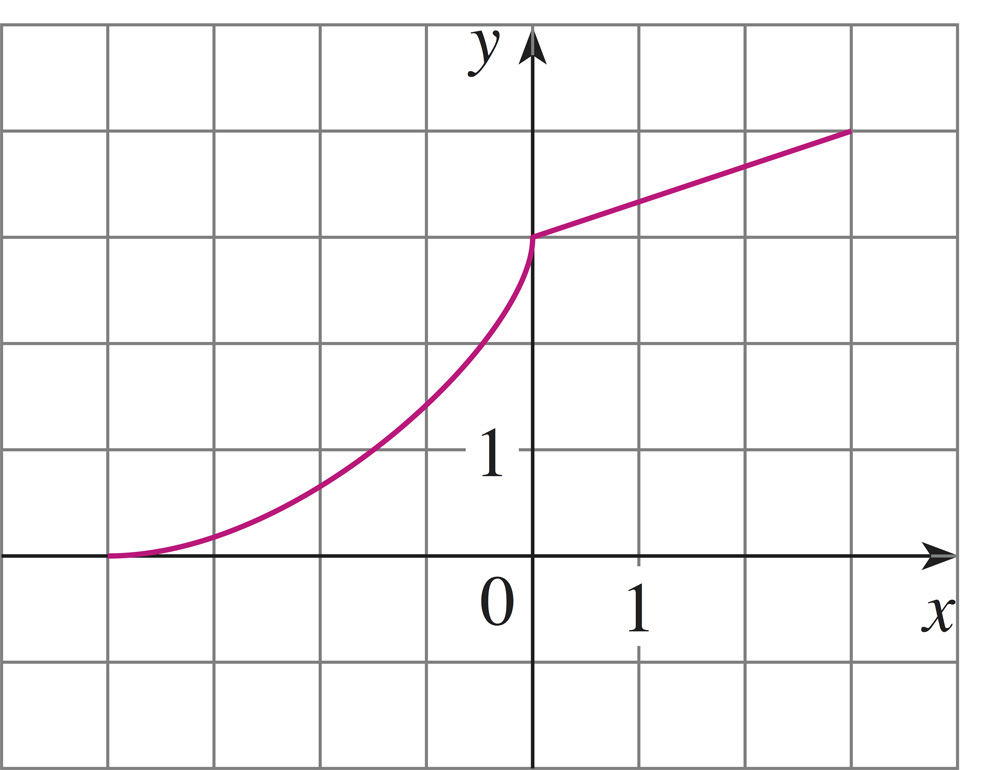
\includegraphics[scale=4]{1Rev_10Stewart8Ed.jpg}
	\part[2] $y=2-f(x)$
	\vspace{2.5pc}
	
	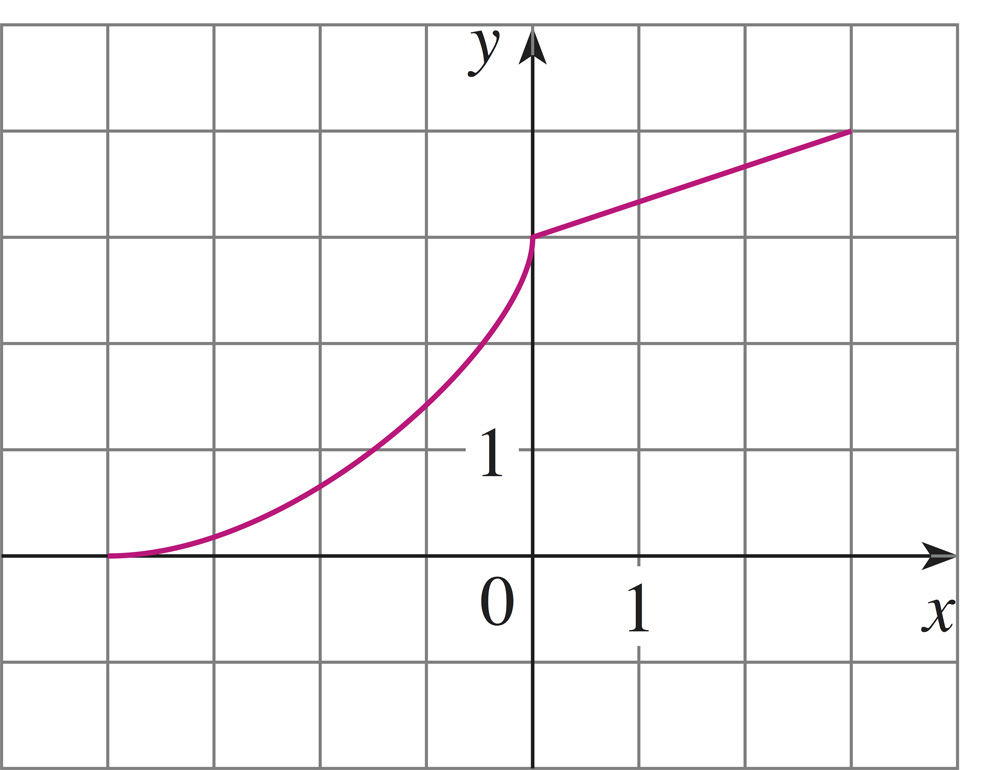
\includegraphics[scale=4]{1Rev_10Stewart8Ed.jpg}
	\part[2] $y=f\1(x)$
	\vspace{2.5pc}
	
	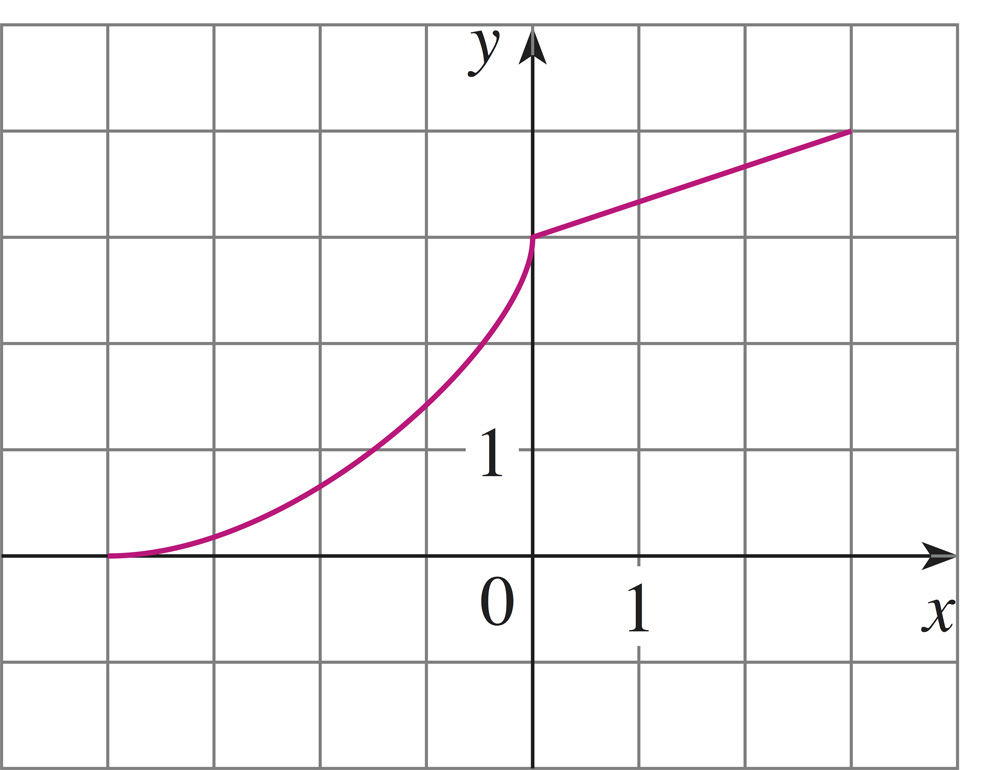
\includegraphics[scale=4]{1Rev_10Stewart8Ed.jpg}
	%\part $y=-f(x)$
	%
	%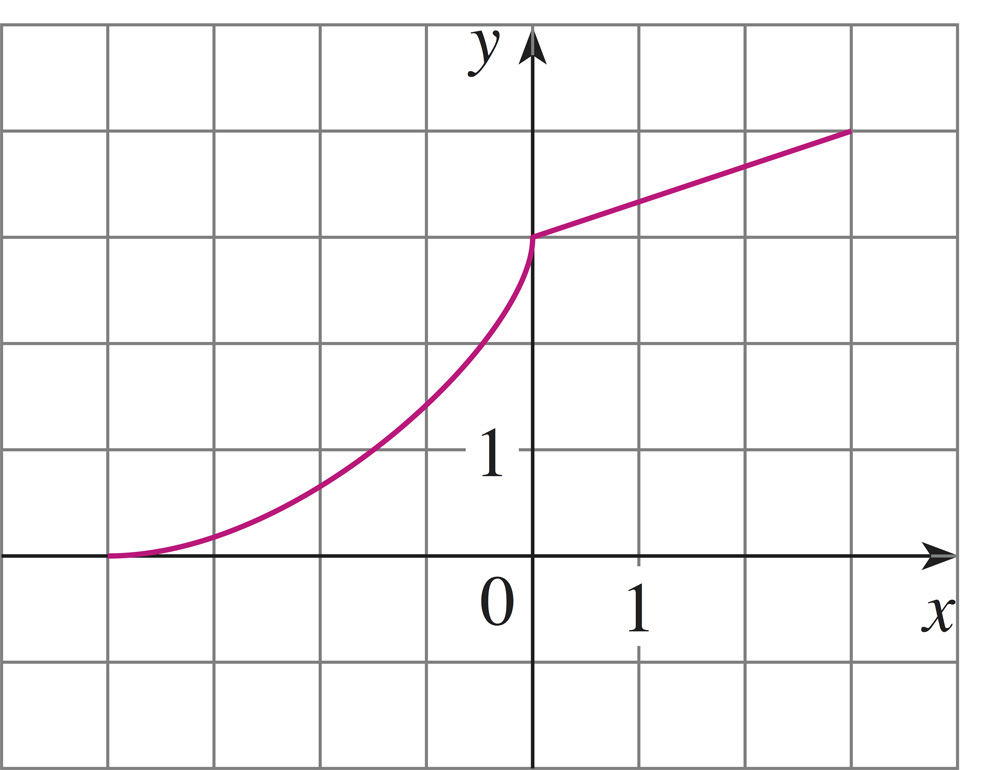
\includegraphics[scale=4]{1Rev_10Stewart8Ed.jpg}
	\part[2] $y=\frac{1}{2}f(x)-1$
	\vspace{2.5pc}
	
	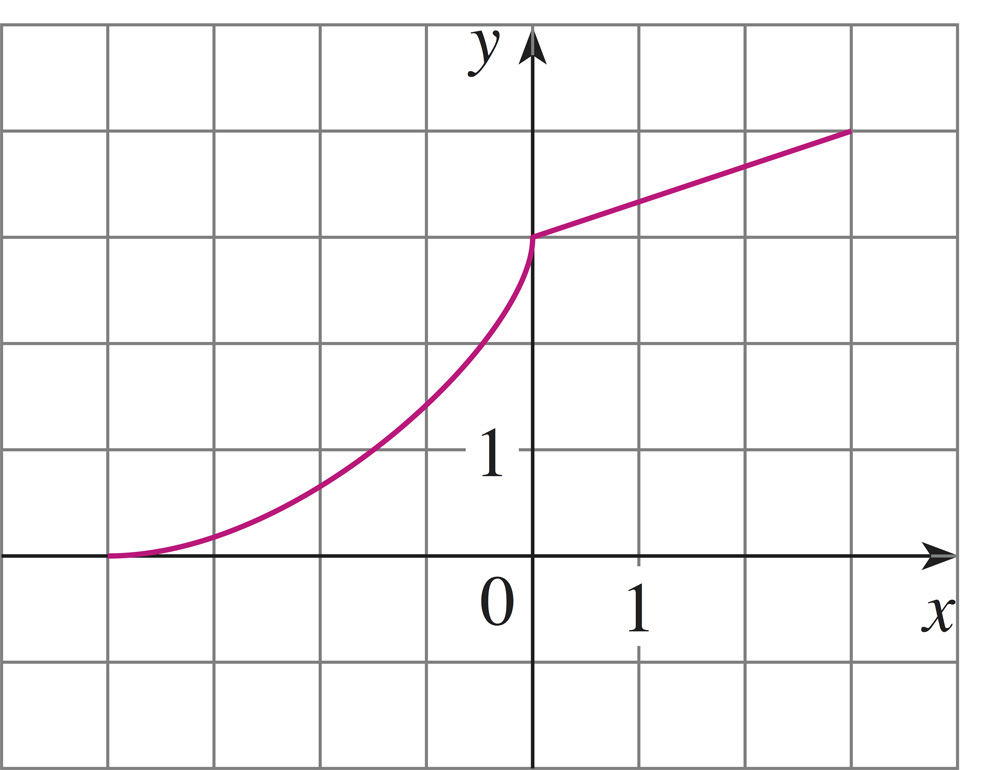
\includegraphics[scale=4]{1Rev_10Stewart8Ed.jpg}
	\part[2] $y=f\1(x+3)$
	\vspace{2.5pc}
	
	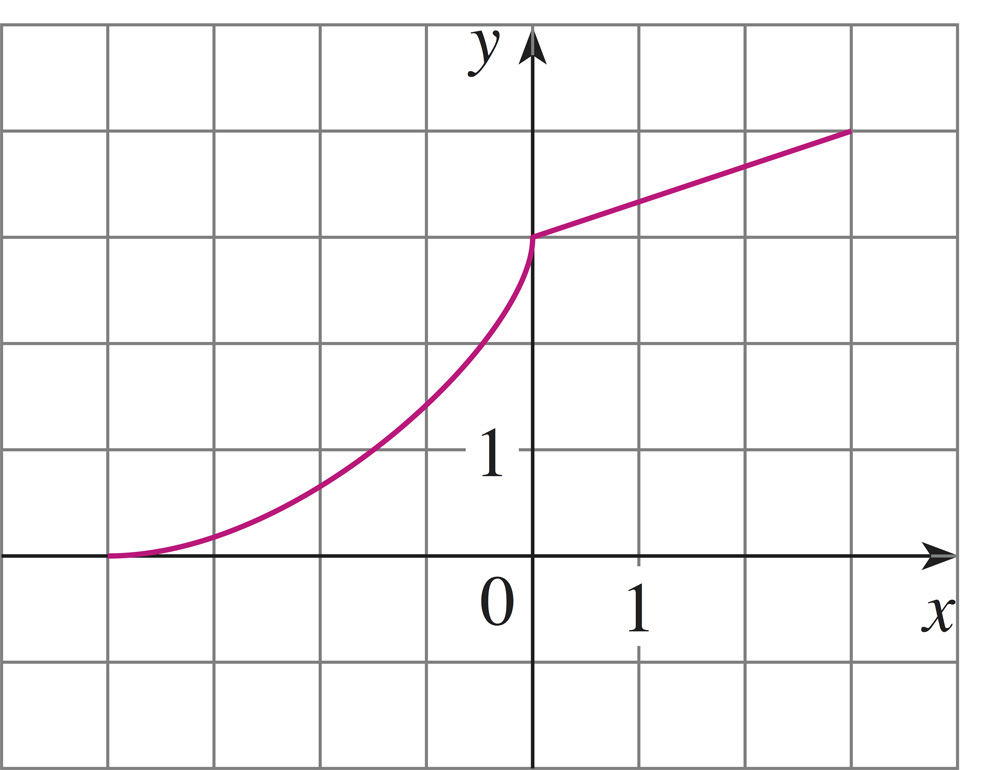
\includegraphics[scale=4]{1Rev_10Stewart8Ed.jpg}
	\end{parts}
\end{multicols}	

\newpage	
% % % % %
\question[2]%{\bf Ch 1 \#22} 
A small-appliance manufacturer finds that it costs \$9000 to produce 1000 toaster ovens a week and \$12,000 to produce 1500 toaster ovens a week.  Express the cost as a function of the number of toaster ovens produced per week, assuming that it is linear. 	
\vspace{5pc}

% % %
\question[3]%{\bf Ch 1 \#24} 
Given $f(x)=\frac{x+1}{2x+1}$, find the inverse function $f\1(x)$.
\vspace{10pc}

% % % 
%\question%{\bf Ch 1 \#26} 
%Solve each equation for $x$.
%\begin{multicols}{2}
%	\begin{parts}
%	\part[1] $e^x=5$
%	\vspace{2pc}
%	
%	\part[1] $e^{e^x}=2$
%	\vspace{2pc}
%	
%	\part[1] $\ln x=2$
%	\vspace{2pc}
%	
%	\part[1] $\arctan x=1$
%	\vspace{2pc}
%	\end{parts}
%\end{multicols}

%\newpage
% % % % %	
\question Evaluate each of the limits.  You must your work and/or justify your answers.
	\begin{parts}
	\part[3]%{\bf Ch 2 \#6} 
	$\lim_{x\to1^+}\frac{x^2-9}{x^2+2x-3}$
	\vspace{5pc}
	
	\part[3]%{\bf Ch 2 \#8} 
	$\lim_{v\to 4^+}\frac{4-v}{|4-v|}$
	\vspace{5pc}
	
	\part[3]%{\bf Ch 2 \#14} 
	$\lim_{x\to -\infty}\frac{\sqrt{x^2-9}}{2x-6}$
	\vspace{5pc}
	
	\part[3]%{\bf Ch 2 \#18} 
	$\lim_{x\to\infty}e^{x-x^2}$
	\vspace{5pc}
	%\part{\bf Ch 2 \#20} $\lim_{x\to 1}\left(\frac{1}{x-1}-\frac{1}{x^2-3x+2}\right)$
	\end{parts}

% % % 	
\question[3]%{\bf Ch 2 \#44} 
The graph of $f$ is shown.  Sketch the graph of $f'$ on the same axes.
\begin{center}
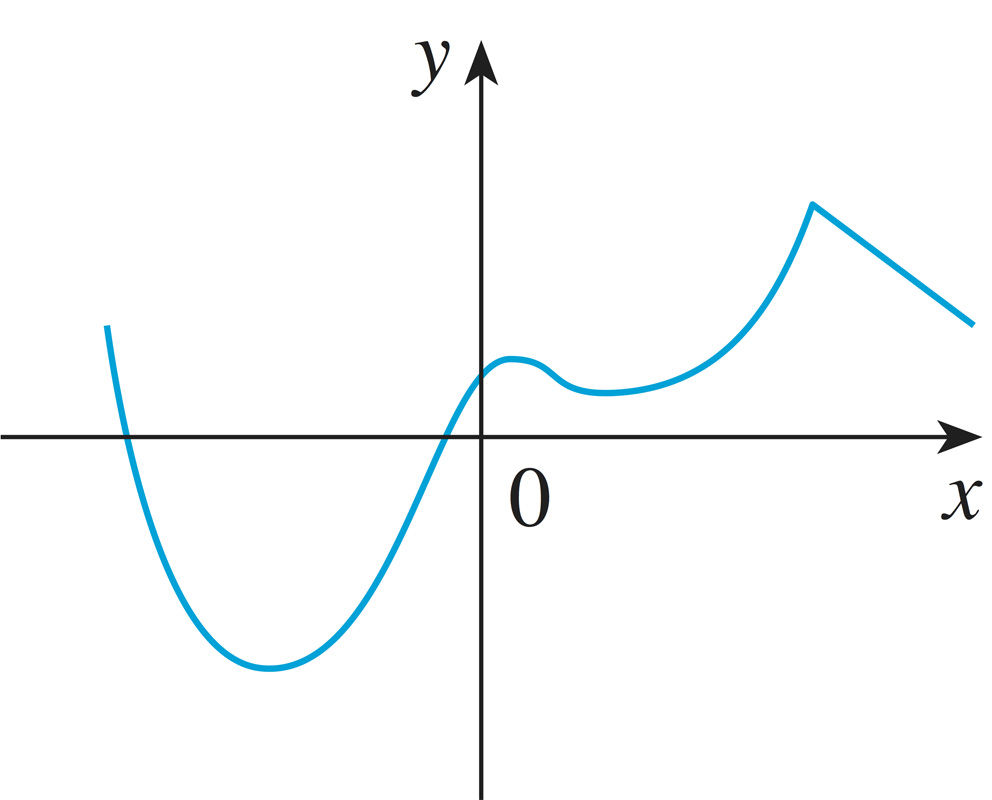
\includegraphics[scale=5]{2Rev_44Stewart8Ed.jpg}
\end{center}
	
% % % 
\question[3]%{\bf Ch 3 \#8}
Use implicit differentiation of the equation $xe^y=y\sin x$ to find $\frac{dy}{dx}$.
\vspace{8pc}

%\newpage
% % % % % 	
\question Find $y'$.  Do not simplify.
%\begin{multicols}{2}	
	\begin{parts}
	\part[2]%{\bf Ch 3 \#20} 
	$y=e^{x\sec x}$
	\vspace{5pc}
	
	%\part{\bf Ch 3 \#26} $y=\sqrt{\sin{\sqrt x}}$
	%\vspace{5pc}
	
	\part[2]%{\bf Ch 3 \#34} 
	$y=10^{\tan{\pi\theta}}$
	\vspace{5pc}
	
	\part[2]%{\bf Ch 3 \#38} 
	$y=\arctan\left(\arcsin x\right)$
	\vspace{5pc}
	%\part{\bf Ch 3 \#40} $xe^y=y-1$
	
	\part[3]%{\bf Ch 3 \#50} 
	$y=\sin^2\left(\cos{\sqrt{\pi x}}\right)$
	\vspace{5pc}
	\end{parts}
%\end{multicols}
	
% % % 
%\question{\bf Ch 3 \#60} Find equations of the tangent line and normal line \textit{(recall, the normal line to a curve with slope $m$ has slope $\textstyle -\frac{1}{m}$)} to the curve $x^2+4xy+y^2=13$ at the point $(0,2)$. 	
%\vspace{10pc}

% % % 
%\question{\bf Ch 3 \#66} Find the points on the ellipse $x^2+2y^2=1$ where the tangent line has slope 1.

% % %
\question Find $f'$ in terms of $g'$.
\begin{multicols}{2}
	\begin{parts}
	\part[1]%{\bf Ch 3 \#72} 
	$f(x)=g(x^2)$
	\vspace{3pc}
	
	\part[1]%{\bf Ch 3 \#74} 
	$f(x)=g(g(x))$
	\vspace{3pc}
	
	\part[1]%{\bf Ch 3 \#76} 
	$f(x)=e^{g(x)}$
	\vspace{3pc}
	
	\part[1]%{\bf Ch 3 \#78} 
	$f(x)=g(\ln x)$
	\vspace{3pc}
	\end{parts}
\end{multicols}

%\newpage
% % % % %
\question[2]%{\bf Ch 3 \#80} 
Find $h'$, given that $h(x)=\sqrt{\frac{f(x)}{g(x)}}$.
\vspace{3pc}

%\question{\bf Ch 3 \#90} The volume of a right circular cone is $V=\frac{1}{3}\pi r^2h$, where $r$ is the radius of the base and $h$ is the height.
%	\begin{parts}
%	\part Find the rate of change of the volume with respect to the height if the radius is constant.
%	\part Find the rate of change of the volume with respect to the radius if the height is constant.
%	\end{parts}

%\newpage
% % % % % 	
\question%{\bf Ch 3 \#94} 
\textit{In this problem, round to one decimal place.  If you do not have a calculator, write the exact number that you would plug in to a calculator to get the answer.}  Cobalt-60 has a half-life of 5.24 years.
	\begin{parts}
	\part[2] Find the mass that remains from a 100-mg sample after 20 years.
	\vspace{5pc}	
	
	\part[2] How long would it take for the 100-mg sample to decay to 1 mg?
	\vspace{5pc}
	\end{parts}

% % % 	
\question%{\bf Ch 3 \#98} 
A paper cup has the shape of a cone with height 10 cm and radius 3 cm (at the top).  The contents of the cup also form a cone shape with radius $r$ and height $h$.  The volume of the contents of the cup is given by the formula $V=\frac{1}{3}\pi r^2h$.  
	\begin{parts}
	\part[2] Use similar triangles to find an equation relating $r$ and $h$.  You may find it helpful to draw a diagram of the cup with some water in it.
	\vspace{8pc}

	\part[2] If water is poured into the cup at a rate of 2 cm$^3$/s, how fast is the water level rising when the water is 5 cm deep?	
	\vspace{10pc}
	\end{parts}

%\newpage
% % % % %	
%\question{\bf Ch 4 \#16} Sketch the graph of a function that satisfies the given conditions.
%\begin{multicols}{2}
%	\begin{itemize}
%	\item $f(0)=0$
%	\item $f$ is continuous and even
%	\item $f'(x)=2x$ if $0<x<1$
%	\item $f'(x)=-1$ if $1<x<3$
%	\item $f'(x)=1$ if $x>3$
%	\end{itemize}	
%\end{multicols}
\vspace{1pc}

% % %	
\question%{\bf Ch 4 \#48} 
Let $y=ax^3+bx^2$.
	\begin{parts}
	\part[3] For what values of the constants $a$ and $b$ is $(1,3)$ a possible point of inflection of the curve $y=ax^3+bx^2$?  \textit{Hint: To solve this problem you need two equations to find the two unknowns.}
	\vspace{8pc}
	
	\part[2] Is $(1,3)$ an actual inflection point of the curve?  You \textit{must} justify your answer.
	\vspace{8pc}
	\end{parts}

% % %	
\question[3]%{\bf Ch 4 \#50}
Find two positive integers such that the sum of the first number and four times the second number is 1000 and the product of the numbers is as large as possible. 	\textit{You must provide justification for why your critical point is indeed a max.}
\vspace{10pc}

\newpage
% % % % %	
\question[3]%{\bf Ch 4 \#74} 
A particle is moving with acceleration function $a(t)=\sin t+3\cos t$.  Its initial velocity is $v(0)=2$ and its initial position is $s(0)=0$.  Find its position function $s(t)$.
\vspace{12pc}

% % % 
\question[2]%{\bf Ch 5 \#9} 
The graph of $f$ consists of the three line segments shown.  If $g(x)=\int_0^xf(t)\ dt$, find $g(4)$ and $g'(4)$.
\begin{center}
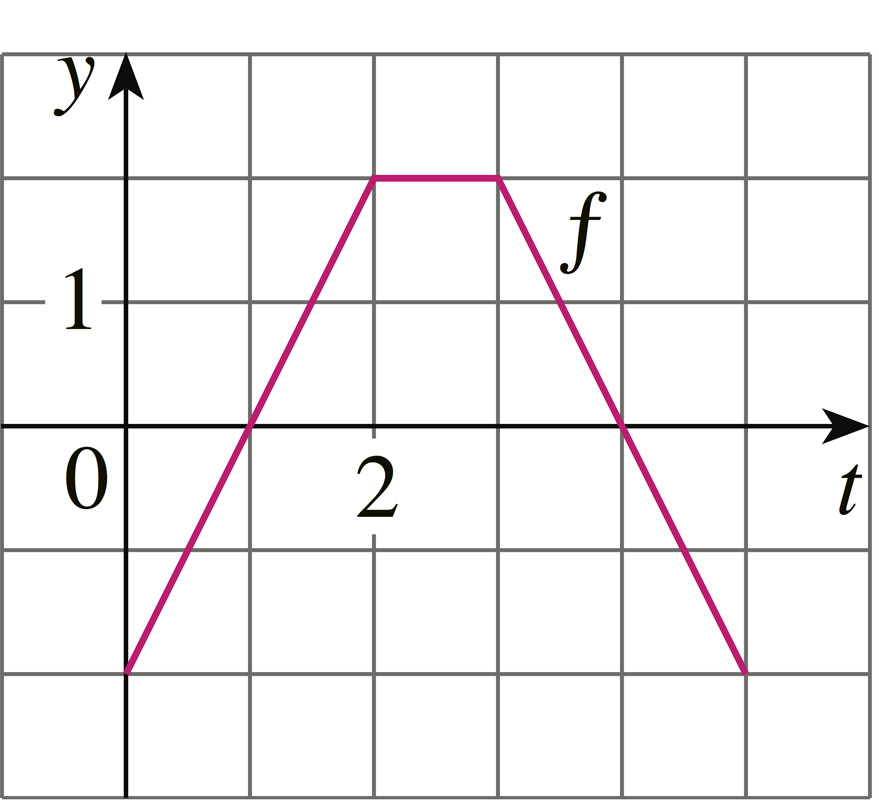
\includegraphics[scale=4]{5Rev_9Stewart8Ed.jpg}
\end{center}

%\newpage
% % % % %
\question Evaluate each of the integrals.
	\begin{parts}
	\part[2]%{\bf Ch 5 \#26} 
	$\int_1^{10}\frac{x}{x^2-4}\ dx$
	\vspace{7pc}
	
	\part[2]%{\bf Ch 5 \#30} 
	$\int \sin x\cos(\cos x)\ dx$
	\vspace{7pc}
	\end{parts}
	
% % % 
\question[2]%{\bf Ch 5 \#48} 
Find the derivative of the function
\[
g(x)=\int_1^{\sin x}\frac{1-t^2}{1+t^4}\ dt.
\] 	
\vspace{5pc}

% % % 
\question[2]%{\bf Ch 5 \#68} 
Suppose $h$ is a function such that $h(1)=-2$, $h'(1)=2$, $h''(1)=3$, $h(2)=6$, $h'(2)=5$, $h''(2)=13$, and $h''$ is continuous everywhere.  Evaluate $\int_1^2h''(u)\ du$.

% % % % %
\end{questions}

\end{document}